% Source: Weinberg GR, physical PDF pp. 339--347
%         (printed pp. 317--325).
% Coverage: Section 11.4, Neutron Stars; equations (11.4.1)--(11.4.29).
% Figures/tables/footnotes: Figure 11.2; reference callouts 8, 10--22.
% Status: source-reviewed and compile-clean.
% Uncertainties: none.

\subsection{Neutron Stars}\label{sec:11.4}

We saw in the last section that a white-dwarf star supported by the pressure
of cold degenerate electrons cannot be in equilibrium if its mass is greater
than the Chandrasekhar limit, about
\(\hbar^{3/2}/(m_N^2G^{3/2})\). Also, the gravitational potential at the
surface of such a star cannot be greater than about \(m_e/m_N\), so general
relativity plays no role in its structure.

Continuing our search for astrophysical applications of general relativity,
let us ask what happens when a star whose mass is above the Chandrasekhar limit
reaches the end of its thermonuclear evolution and grows cold. Its internal
pressure then fails to support it, and it collapses. One possibility is that
the star will simply go on collapsing forever, in which case general relativity
will certainly come into play. Another possibility is that the star will
become so heated during its collapse that it will explode, becoming a
supernova. It might then blow off enough matter so that its mass drops below
the Chandrasekhar limit. It is believed that in this case the highly compressed
remnant does not find its quietus as a white dwarf, but rather becomes a
superdense neutron star.\hyperref[ch11-ref-10]{\textsuperscript{10}}
(See Figure~\ref{fig:11.2}.)

% Source: Weinberg GR, physical PDF p. 340 (printed p. 318).
% Coverage: Figure 11.2, configurations of stellar equilibrium.
% Status: source plot extracted at source resolution; source-reviewed.
% Uncertainties: none.

\begingroup
\renewcommand{\thefigure}{11.2}
\begin{figure}[htbp]
  \centering
  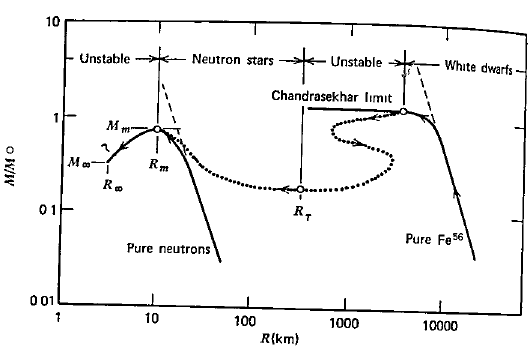
\includegraphics[width=0.83\textwidth]{figures/chapter11/fig11-02.png}
  \caption{Configurations of stellar equilibrium. The solid curves on the
  left and right represent the Oppenheimer--Volkoff%
  \hyperref[ch11-ref-10]{\textsuperscript{10}} solution for a pure neutron
  star and the Chandrasekhar%
  \hyperref[ch11-ref-8]{\textsuperscript{8}} solution for a pure
  \(\mathrm{Fe}^{56}\) white-dwarf star, respectively. The dashed lines give
  the extrapolated nonrelativistic solutions in these two cases. The dotted
  line represents the interpolating solution of Harrison, Thorne, Wakano, and
  Wheeler,\hyperref[ch11-ref-12]{\textsuperscript{12}} which takes into
  account the shift in chemical composition from \(\mathrm{Fe}^{56}\) to
  neutrons. Arrows indicate the direction of increasing central density. As
  shown in Theorem~1, the various transitions between stability and
  instability occur at the maxima and minima of \(M\), marked here with small
  circles.}
  \label{fig:11.2}
\end{figure}
\endgroup


A neutron star is like a white dwarf, except that it consists almost entirely
of ``cold'' degenerate neutrons, all electrons and protons having been
converted into neutrons through the reaction
\[
  p+e^-\longrightarrow n+\nu,
\]
the neutrinos escaping the star. Enough electrons and protons must remain so
that the Pauli principle prevents neutron beta decay,
\(n\to p+e^-+\bar\nu\); this sets a lower limit on the mass of stable neutron
stars, to be evaluated below.

Neutron stars of low mass are much like white dwarfs of the same mass, except
that neutron degeneracy pressure replaces electron degeneracy pressure, and
thus \(m_e\) should be replaced in all formulas with \(m_n\) (and \(\mu\)
should be set equal to unity). Thus, by noting how \(m_e\) enters in the
formulas \eqref{eq:11.3.44}--\eqref{eq:11.3.47} for small white dwarfs, we
can immediately conclude that a neutron star of small mass will have a central
density higher than that of a white dwarf with the same mass (and \(\mu=2\))
by a factor \((2m_n/m_e)^3=3.1\times10^9\), and will have a radius smaller by
a factor \(m_n/(2m_e)=920\).

The electrons in a white dwarf will begin to be relativistic when its mass
becomes comparable to the theoretical upper limit, given by
Eq.~\eqref{eq:11.3.49}. Since \(m_e\) does not enter in
Eq.~\eqref{eq:11.3.49}, we expect that the neutrons in a neutron star will
begin to be relativistic at just such masses, that is, when \(M\) is of order
\(M_\odot\). However, at this point the analogy between white dwarfs and
neutron stars breaks down. For one thing, the total energy density \(\rho\) of
a white dwarf is always dominated by the rest-mass density of its
nonrelativistic nucleons, whereas a neutron star with mass of order
\(M_\odot\) will consist of nucleons whose kinetic energies are comparable
with their rest masses. Another difference that is even more interesting is
that, whereas a white dwarf whose electrons are moderately relativistic will
have a surface gravitational potential \(GM/R\) of order \(m_e/m_n\), a
neutron star of equal mass will have a surface potential roughly of order
unity. Thus general relativity will necessarily play a role in the theory of
the more massive neutron stars.

In order to formulate the quantitative theory of neutron stars, we begin by
writing down expressions for the total energy density and pressure of an ideal
Fermi gas of neutrons with maximum momentum \(k_F\):
\begin{align}
  \rho
  &=
  \frac{8\pi}{(2\pi\hbar)^3}
  \int_0^{k_F}(k^2+m_n^2)^{1/2}k^2\,dk
  =
  3\rho_c\int_0^{k_F/m_n}(u^2+1)^{1/2}u^2\,du,
  \tag{11.4.1}\label{eq:11.4.1}\\
  p
  &=
  \frac{8\pi}{3(2\pi\hbar)^3}
  \int_0^{k_F}\frac{k^2}{(k^2+m_n^2)^{1/2}}k^2\,dk
  =
  \rho_c\int_0^{k_F/m_n}(u^2+1)^{-1/2}u^4\,du,
  \tag{11.4.2}\label{eq:11.4.2}
\end{align}
where now (in c.g.s.\ units)
\begin{equation}
  \rho_c
  \equiv
  \frac{8\pi m_n^4c^3}{3(2\pi\hbar)^3}
  =
  6.11\times10^{15}\ \mathrm{g\,cm^{-3}}.
  \tag{11.4.3}\label{eq:11.4.3}
\end{equation}
By eliminating \(k_F/m_n\) in Eqs.~\eqref{eq:11.4.1} and
\eqref{eq:11.4.2}, we obtain the equation of state in the form
\begin{equation}
  \frac p{\rho_c}
  =
  F\left(\frac{\rho}{\rho_c}\right),
  \tag{11.4.4}\label{eq:11.4.4}
\end{equation}
with \(F\) a definite transcendental function. The structure of a neutron star
with given central density \(\rho(0)\) is to be calculated by solving
Eq.~\eqref{eq:11.1.13} with \(p\) given as a function of \(\rho\) by
Eq.~\eqref{eq:11.4.4}. Since the only dimensional quantities in these
equations are \(\rho(0)\), \(\rho_c\), and \(G\), the solution must give the
mass and radius as functions of \(\rho(0)\) of the form
\begin{align}
  M&=M_0f\left(\frac{\rho(0)}{\rho_c}\right),
  \tag{11.4.5}\label{eq:11.4.5}\\
  R&=R_0g\left(\frac{\rho(0)}{\rho_c}\right),
  \tag{11.4.6}\label{eq:11.4.6}
\end{align}
where (in c.g.s.\ units)
\begin{align}
  R_0&=c(8\pi G\rho_c)^{-1/2}=3.0\ \mathrm{km},
  \tag{11.4.7}\label{eq:11.4.7}\\
  M_0&=\frac{c^2R_0}{G}=2.0M_\odot,
  \tag{11.4.8}\label{eq:11.4.8}
\end{align}
and \(f\) and \(g\) are unknown dimensionless functions. This problem, like
that of the white dwarfs, is analytically tractable only for very large and
very small central densities.

For \(\rho(0)\ll\rho_c\) we can use the analogy with white dwarfs discussed
above, and conclude from Eqs.~\eqref{eq:11.3.46} and \eqref{eq:11.3.47}
that
\begin{equation}
  \begin{split}
  M
  &=
  \frac12\left(\frac{3\pi}{8}\right)^{1/2}(2.71406)
  \left(\frac{\hbar^{3/2}}{m_n^2G^{3/2}}\right)
  \left(\frac{\rho(0)}{\rho_c}\right)^{1/2}\\
  &=
  \frac12(2.71406)M_0
  \left(\frac{\rho(0)}{\rho_c}\right)^{1/2},
  \end{split}
  \tag{11.4.9}\label{eq:11.4.9}
\end{equation}
\begin{equation}
  \begin{split}
  R
  &=
  \left(\frac{3\pi}{8}\right)^{1/2}(3.65375)
  \left(\frac{\hbar^{3/2}}{m_n^2G^{1/2}}\right)
  \left(\frac{\rho_c}{\rho(0)}\right)^{1/6}\\
  &=
  (3.65375)R_0
  \left(\frac{\rho_c}{\rho(0)}\right)^{1/6},
  \end{split}
  \tag{11.4.10}\label{eq:11.4.10}
\end{equation}
with \(\rho_c\) now given by Eq.~\eqref{eq:11.4.3}.

For \(\rho(0)\gg\rho_c\), the neutrons near the center of the star have
\(k_F\gg m_n\), so Eqs.~\eqref{eq:11.4.1} and \eqref{eq:11.4.2} give
\[
  \rho=\frac{3\rho_c}{4}\left(\frac{k_F}{m_n}\right)^4,
  \qquad
  p=\frac{\rho_c}{4}\left(\frac{k_F}{m_n}\right)^4,
\]
and therefore
\begin{equation}
  p=\frac{\rho}{3},
  \tag{11.4.11}\label{eq:11.4.11}
\end{equation}
as would be expected for a gas of highly relativistic particles. Using this
equation of state in the fundamental differential equation
\eqref{eq:11.1.13} gives
\begin{equation}
  -r^2\rho'(r)
  =
  4G\mathcal{M}(r)\rho(r)
  \left[1+\frac{4\pi r^3\rho(r)}{3\mathcal{M}(r)}\right]
  \left[1-\frac{2G\mathcal{M}(r)}r\right]^{-1}.
  \tag{11.4.12}\label{eq:11.4.12}
\end{equation}
Amazingly, we can find an exact solution of this
equation:\hyperref[ch11-ref-11]{\textsuperscript{11}}
\begin{equation}
  \rho(r)=\frac{3}{56\pi Gr^2},
  \tag{11.4.13}\label{eq:11.4.13}
\end{equation}
corresponding to the limit \(\rho(0)\to\infty\). However, even in the limit
of infinite central density, this \(\rho(r)\) will drop below \(\rho_c\) at a
radius \(r\) of order \(R_0\), so that the equation of state
\eqref{eq:11.4.11} is not valid for the outer layers of \emph{any} neutron
star. To deal with the crust of nonrelativistic neutrons, it is necessary to
solve the full equation \eqref{eq:11.1.13} using the equation of state
\eqref{eq:11.4.4}; the condition of infinite central density is imposed by
\eqref{eq:11.4.13} for \(r\ll R_0\). We shall not do this here; the important
points are that the solution has a finite radius \(R\) where \(\rho\)
vanishes, and that the mass \(M\) within this radius is finite, because the
singularity in Eq.~\eqref{eq:11.4.13} is integrable at \(r=0\). Thus the
mass and radius of a neutron star approach finite limits as
\(\rho(0)\to\infty\). Numerical solution of the fundamental equation
\eqref{eq:11.1.13} gives these limits
as\hyperref[ch11-ref-10]{\textsuperscript{10}}
\begin{equation}
  M_\infty=0.171M_0,\qquad R_\infty=1.06R_0.
  \tag{11.4.14}\label{eq:11.4.14}
\end{equation}

There remains the question of stability. For \(\rho(0)\ll\rho_c\), a pure
neutron star is simply a Newtonian polytrope with \(\gamma=5/3\) (like a small
white dwarf) and is therefore stable. (See Section~\ref{sec:11.3}.)
Equation~\eqref{eq:11.4.9} shows that \(M\) is a monotonically increasing
function of \(\rho(0)\) for these small central densities. If \(M\) continues
to increase monotonically to the value \(M_\infty\), then no transition to
instability can occur, according to Theorem~1 of Section~\ref{sec:11.2}. But
Eq.~\eqref{eq:11.4.9} shows that when \(\rho(0)=0.016\rho_c\) (which is
small enough for Eq.~\eqref{eq:11.4.9} to be a good approximation), the mass
\(M\) is already greater than \(M_\infty\). Thus we expect that \(M\) rises
to a maximum value \(M>M_\infty\) at some central density \(\rho_m\) of order
\(\rho_c\), and then drops to the value \(M_\infty\) at infinite central
density. This expectation is confirmed by detailed
calculation\hyperref[ch11-ref-10]{\textsuperscript{10}} using
Eqs.~\eqref{eq:11.1.13} and
\eqref{eq:11.4.1}--\eqref{eq:11.4.3}. The mass \(M\) of a pure ideal-gas
neutron star reaches a maximum
\begin{equation}
  M_m=0.36M_0=0.7M_\odot
  \tag{11.4.15}\label{eq:11.4.15}
\end{equation}
at a radius
\begin{equation}
  R_m=3.2R_0=9.6\ \mathrm{km}.
  \tag{11.4.16}\label{eq:11.4.16}
\end{equation}
Since this is a point where \(\partial M/\partial\rho(0)\) vanishes, we
expect a transition here from stability to instability with respect to radial
oscillations. Thus Eqs.~\eqref{eq:11.4.15} and \eqref{eq:11.4.16}
characterize a neutron star with the greatest mass and central density allowed
by the requirement that the star be stable. The mass
\eqref{eq:11.4.15} is known as the \emph{Oppenheimer--Volkoff limit}. Note
that the fractional redshift of a spectral line emitted from the surface of
such a neutron star is
\begin{equation}
  z\equiv\frac{\Delta\lambda}{\lambda}
  =
  B^{-1/2}(R_m)-1
  =
  \left(1-\frac{2M_mG}{R_m}\right)^{-1/2}-1
  =
  0.13.
  \tag{11.4.17}\label{eq:11.4.17}
\end{equation}
[See Eqs.~\eqref{eq:3.5.3}, \eqref{eq:11.1.1}, and
\eqref{eq:11.1.17}.] Evidently general relativity is just beginning to be
important for the most massive stable neutron stars.

Of course, a neutron star cannot consist purely of neutrons, if only because
we need a Fermi sea of electrons so that the Pauli exclusion principle can
block the neutrons' beta decay. In order to get a first taste of the chemical
composition in a neutron star, let us consider the equilibrium among neutrons,
protons, and electrons. The energy density and number density of each one of
these three Fermi gases are given (for \(i=n,p,e\)) by
\begin{align}
  \rho_i
  &=
  \frac{8\pi}{(2\pi\hbar)^3}
  \int_0^{k_{F,i}}(k^2+m_i^2)^{1/2}k^2\,dk,
  \tag{11.4.18}\label{eq:11.4.18}\\
  n_i
  &=
  \frac{8\pi}{(2\pi\hbar)^3}
  \int_0^{k_{F,i}}k^2\,dk
  =
  \frac{k_{F,i}^3}{3\pi^2\hbar^3}.
  \tag{11.4.19}\label{eq:11.4.19}
\end{align}
At any given point in the star, the reactions
\(n\to p+e^-+\bar\nu\) and \(p+e^-\to n+\nu\) can convert neutrons into
protons and vice versa. (The neutrinos escape.) These reactions preserve the
total number density of baryons,
\begin{equation}
  n_n+n_p=n_B\qquad(\text{fixed}),
  \tag{11.4.20}\label{eq:11.4.20}
\end{equation}
and preserve charge neutrality,
\begin{equation}
  n_p-n_e=0.
  \tag{11.4.21}\label{eq:11.4.21}
\end{equation}
But with \(n_B\) fixed, the total energy density may be expressed in terms of
\(n_n\) alone:
\begin{equation}
  \begin{aligned}
  \rho
  &=
  \rho_n+\rho_e+\rho_p\\
  &=
  3C^{-3}\bigg\{
    \int_0^{Cn_n^{1/3}}(k^2+m_n^2)^{1/2}k^2\,dk\\
  &\qquad
    +\int_0^{C(n_B-n_n)^{1/3}}(k^2+m_p^2)^{1/2}k^2\,dk\\
  &\qquad
    +\int_0^{C(n_B-n_n)^{1/3}}(k^2+m_e^2)^{1/2}k^2\,dk
  \bigg\},
  \end{aligned}
  \tag{11.4.22}\label{eq:11.4.22}
\end{equation}
where
\[
  C=(3\pi^2\hbar^3)^{1/3}.
\]
Chemical equilibrium is reached when this function is a minimum, that is, at
\[
  \begin{aligned}
  0=\frac{d\rho}{dn_n}
  ={}&
  (C^2n_n^{2/3}+m_n^2)^{1/2}\\
  &-(C^2[n_B-n_n]^{2/3}+m_p^2)^{1/2}\\
  &-(C^2[n_B-n_n]^{2/3}+m_e^2)^{1/2}.
  \end{aligned}
\]
We can solve for \(n_p=n_B-n_n\) as a function of \(n_n\). The nucleon mass
difference \(Q=m_n-m_p\) and the electron mass \(m_e\) are of comparable
magnitude and very much less than \(m_n\), so the result can be written more
simply as
\begin{equation}
  \frac{n_p}{n_n}
  =
  \frac18
  \left\{
    \frac{
      1+\dfrac{4Q}{m_n}
        \left(\dfrac{\rho_c}{m_nn_n}\right)^{2/3}
      +\dfrac{4(Q^2-m_e^2)}{m_n^2}
        \left(\dfrac{\rho_c}{m_nn_n}\right)^{4/3}
    }{
      1+\left(\dfrac{\rho_c}{m_nn_n}\right)^{2/3}
    }
  \right\}^{3/2}.
  \tag{11.4.23}\label{eq:11.4.23}
\end{equation}
Here \(\rho_c=m_n^4/C^3\) is the critical density previously defined in
Eq.~\eqref{eq:11.4.3}.

The condition for the neutrons to be stable against beta decay is that the
electron Fermi sea should be filled up to a momentum greater than the maximum
momentum \(k_{\max}\) of the electron emitted in neutron beta decay:
\begin{equation}
  k_{F,e}>k_{\max},
  \tag{11.4.24}\label{eq:11.4.24}
\end{equation}
where
\begin{equation}
  \begin{split}
  k_{\max}
  &=
  \frac{
    [(m_n^2-m_p^2)^2-2m_e^2(m_n^2+m_p^2)+m_e^4]^{1/2}
  }{2m_n}\\
  &\simeq(Q^2-m_e^2)^{1/2}=1.19\ \mathrm{MeV}.
  \end{split}
  \tag{11.4.25}\label{eq:11.4.25}
\end{equation}
The electron Fermi momentum is given by Eqs.~\eqref{eq:11.4.19} and
\eqref{eq:11.4.21} as
\begin{equation}
  \begin{aligned}
  k_{F,e}^2
  &=
  C^2n_e^{2/3}
  =
  C^2n_p^{2/3}
  \simeq
  m_n^2
  \left(\frac{m_nn_n}{\rho_c}\right)^{2/3}
  \left(\frac{n_p}{n_n}\right)^{2/3}\\
  &=
  \frac{
    \dfrac{m_n^2}{4}
      \left(\dfrac{m_nn_n}{\rho_c}\right)^{4/3}
    +Qm_n\left(\dfrac{m_nn_n}{\rho_c}\right)^{2/3}
    +Q^2-m_e^2
  }{
    \left(\dfrac{m_nn_n}{\rho_c}\right)^{2/3}+1
  }.
  \end{aligned}
  \tag{11.4.26}\label{eq:11.4.26}
\end{equation}
This is smallest at \(n_n=0\), where \(k_{F,e}\) barely equals the value
\(k_{\max}\). Hence the condition \eqref{eq:11.4.24} for neutron beta
stability is indeed satisfied for any positive neutron density.

The proton-neutron ratio \eqref{eq:11.4.23} is large and decreasing for very
small neutron densities, reaches a minimum for \(m_nn_n\) equal to the
transition density
\begin{equation}
  \rho_T
  \simeq
  \rho_c
  \left[\frac{4(Q^2-m_e^2)}{m_n^2}\right]^{3/4}
  =
  1.28\times10^{-4}\rho_c,
  \tag{11.4.27}\label{eq:11.4.27}
\end{equation}
where
\begin{equation}
  \left(\frac{n_p}{n_n}\right)_{\min}
  \simeq
  \left[
    \frac{Q+\tfrac12(Q^2-m_e^2)^{1/2}}{m_n}
  \right]^{3/2}
  =
  0.002,
  \tag{11.4.28}\label{eq:11.4.28}
\end{equation}
and then rises monotonically, reaching the value \(1/8\) for
\(n_nm_n\gg\rho_c\). Stars with a central density somewhat less than the
transition value \eqref{eq:11.4.27} are not really neutron stars at all, but
belong to the extreme high-density branch of the white-dwarf equilibrium
solutions, and are therefore unstable. (See Section~\ref{sec:11.3}.) Thus we
expect there to be some minimum central density of order \(\rho_T\), and some
minimum mass of order
\(3M_\odot(\rho_T/\rho_c)^{1/2}\simeq0.03M_\odot\) [see
Eq.~\eqref{eq:11.4.9}], below which stable neutron stars could not exist.
Detailed calculations\hyperref[ch11-ref-12]{\textsuperscript{12}} show that
the minimum mass of a neutron star is actually about \(0.2M_\odot\).

The small hydrogen contamination in a neutron star is more interesting than
might be thought, because the filling of proton and electron as well as neutron
energy levels will block the decay of various particles besides the neutron
that are normally unstable. For instance, the \(\mu^-\)-meson becomes stable
when \(k_{F,e}>53\ \mathrm{MeV}\), because then the Pauli principle will block
the emission of electrons in the decay process
\(\mu^-\to e^-+\nu+\bar\nu\). According to Eq.~\eqref{eq:11.4.26}, this
happens when the density \(\rho\simeq m_nn_n\) reaches the value
\(0.038\rho_c\), when \(n_p=0.005n_n\). When the density reaches
\(0.107\rho_c\), with \(n_p=0.013n_n\), the electron Fermi momentum reaches
the \(\mu\)-meson mass \(105\ \mathrm{MeV}\), and it becomes energetically
favorable for electrons at the top of the Fermi sea to be converted (say by
collisions) into \(\mu^-\)-mesons, with a neutrino-antineutrino pair escaping
from the star. Thus neutron stars of even moderate mass will be contaminated
with \(\mu^-\)-mesons as well as hydrogen. The same reasoning leads us to
expect that hyperons and various excited states of the nucleons and hyperons
also will be stable and present in small amounts.

This raises an interesting question of principle. For instance, the famous
\(3\)-\(3\) resonance in pion-nucleon scattering may be thought of either as
a manifestation of the pion-nucleon force, or as a particle, the
\(\Delta\) baryon, with a mass \(1236\ \mathrm{MeV}\) and the very short
lifetime \(5.5\times10^{-20}\ \mathrm{s}\). Should we include the \(\Delta\)
in ideal-gas models of neutron stars? Normally one would think not, but for
high enough nucleon density the Pauli principle will block the decays
\(\Delta\to N+\pi\), \(\Delta\to N+\gamma\), and so on, and energetic
considerations will favor the conversion of some neutrons and protons into
\(\Delta\)s. Of course, it is possible that the strong interactions among
nucleons simply rule out any ideal-gas model of a dense neutron star, but it
is also possible that the effects of these forces can be taken into account by
treating a neutron star as an ideal gas of neutrons, protons, electrons,
\(\mu^-\)-mesons, hyperons, and nucleon and hyperon resonances. (See
Section~15.11.)

In any case, it should be clear that the Oppenheimer--Volkoff calculation,
which treats a neutron star as a pure ideal gas of neutrons, must be used with
a good deal of caution when \(\rho(0)\) is comparable with or greater than
\(\rho_c\). Merely including protons and electrons as well as neutrons in an
ideal-gas model does not by itself have a serious effect on the structure of a
neutron star,\hyperref[ch11-ref-12]{\textsuperscript{12}} but nuclear forces
can be quite important. For instance, various detailed calculations yield
values of the maximum stable mass equal to \(0.37M_\odot\),
\hyperref[ch11-ref-13]{\textsuperscript{13}} \(1.95M_\odot\),
\hyperref[ch11-ref-14]{\textsuperscript{14}} and \(2.4M_\odot\).
\hyperref[ch11-ref-15]{\textsuperscript{15}} Even these models are still
highly idealized; a real neutron star is expected to have a crystalline
crust,\hyperref[ch11-ref-16]{\textsuperscript{16}} a superfluid
interior,\hyperref[ch11-ref-17]{\textsuperscript{17}} powerful magnetic
fields,\hyperref[ch11-ref-18]{\textsuperscript{18}} and often a very rapid
rate of rotation.\hyperref[ch11-ref-19]{\textsuperscript{19}}

The discovery\hyperref[ch11-ref-20]{\textsuperscript{20}} in 1967 of
``pulsars,'' stars that emit radiation at various wavelengths in regular
pulses separated by intervals from a few seconds down to \(0.033\ \mathrm{s}\),
suggests that we should look into the possible rotation and vibration periods
of neutron stars and white dwarfs. Equations~\eqref{eq:11.3.37} and
\eqref{eq:11.3.38} show that for all \(\gamma\) except \(6/5\), \(4/3\), or
\(1\), the maximum rotation frequency and the fundamental vibration frequency
of any Newtonian polytrope are both of order \(\sqrt{GM/R^3}\). Presumably
this result holds to within an order of magnitude for any stable neutron star;
in this case the characteristic frequency is greatest when \(M\) and \(R\)
take the values \eqref{eq:11.4.15} and \eqref{eq:11.4.16}, where it has the
value
\begin{equation}
  \left(\frac{GM_m}{R_m^3}\right)^{1/2}
  =
  10^4\ \mathrm{s^{-1}}.
  \tag{11.4.29}\label{eq:11.4.29}
\end{equation}
This is considerably faster than any observed pulsar frequency. It is
currently believed that pulsars are rotating neutron
stars,\hyperref[ch11-ref-21]{\textsuperscript{21}} which begin life with a
rotation frequency near the maximum, of order \(10^4\ \mathrm{s^{-1}}\), but
which subsequently slow down, losing their energy through gravitational and
electromagnetic radiation and through electromagnetic acceleration of charged
particles. (In order to account for the existence of this radiation as well
as for the observed pulses, it is necessary to suppose that the star does not
have circular symmetry about the axis of rotation, as would be the case if its
magnetic poles are offset from its rotation poles.) This interpretation is
supported by the observation that several pulsars are slowing
down.\hyperref[ch11-ref-22]{\textsuperscript{22}}

A white dwarf with the same mass as a neutron star will have a radius larger
by a factor \(m_n/(\mu m_e)\simeq900\), so the fundamental vibration frequency
and the maximum rotation frequency will be smaller than for a neutron star by
a factor \(3\times10^{-5}\). For \(M\) near \(M_m\) this gives a
characteristic frequency smaller than Eq.~\eqref{eq:11.4.29} by this factor,
or about \(0.3\ \mathrm{s^{-1}}\). This is slower than the observed pulse rate
of most pulsars. Pulsars are probably neutron stars, not white dwarfs.
